\section{Results}

%%%%%%%%%%%%%%%%%%%%%%%%%%%%%%%%%%%%%%%%%
%% Spontaneous firing rates and oscillations
\subsection{Cell type-, layer and sublayer-specific spontaneous firing rates and physiological oscillations}
%% Figure: spontaneous firing rates and oscillations
\begin{figure}[!h]  %% bht
\centering
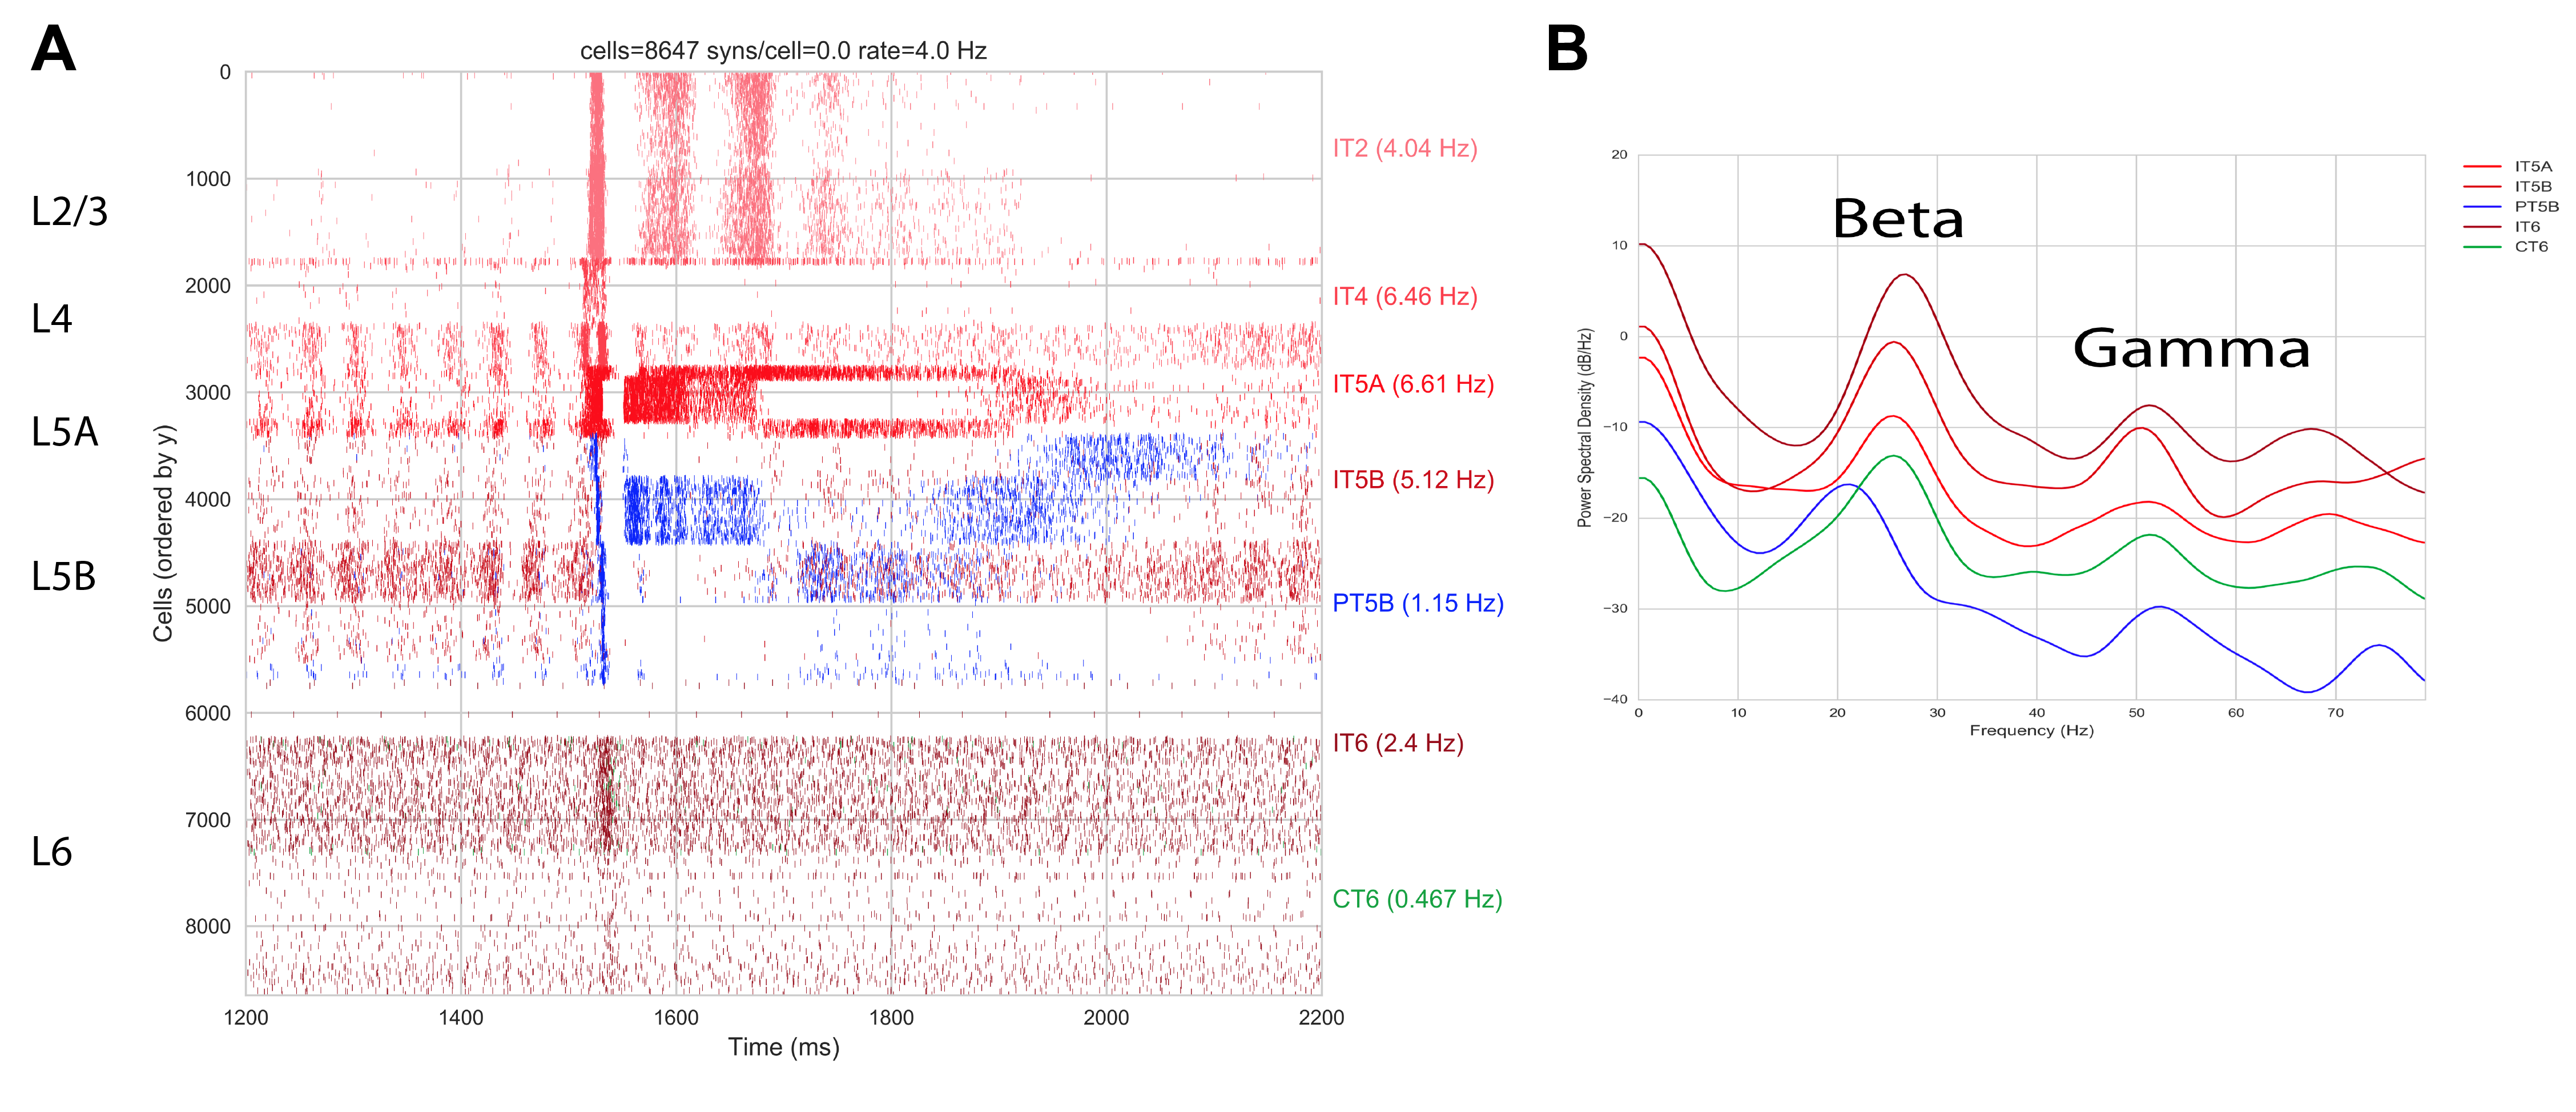
\includegraphics[width=\textwidth]{figs/spont.png}
\caption{{\bf Cell type-, layer and sublayer-specific spontaneous firing rates and physiological oscillatio.}
A) Raster plot with cells arranged by cortical depth. Note higher activity in upper vs lower layer 5B PT cells. 
B) Firing rate power density spectrum.
}
\label{fig_spont}
\end{figure}

\note{B) Firing rates statistics for each population (for comparison with in vivo data).}

%% Firing rates specific to cell, layer, sublayer; comparison with in vivo
Simulations of M1 (\fref{fig_spont}A) exhibit spontaneous firing rates between 0 and 10 Hz for all populations, consistent with the experimental litearature \cite{Isom09,LiDa16}. The sublaminar specificity of connections is evidenced by the gradual decrease of PT activity as cortical depth increases within layer 5B, reflecting experimental observations \cite{Ande10}. The circuit also showed emergence of physiological oscillations in the beta and gamma range (\fref{fig_spont}B)  consistent with in vivo data \cite{Cast13,Rubi06}. These oscillations emerged in the absence of rhythmic external inputs.
\note{Firing rates and coefficient of variation (across cells) for each population (cell types and layers), consistent with in vivo data (\fref{fig_spont}A,B).}
\note{show cortical depth arraged neurons; effect of NCD conn -> upper L5B fire more/first} 

%% Physiological oscillations
\note{Emergence of physiological oscillations in the absence of rhythmic external inputs (beta and gamma peaks), consistent with in vivo data (\fref{fig_spont}C).}
\note{
\cite{Cast13} - rodent M1 produces 7-14Hz oscillations
\cite{Rubi06} - 10-45 Hz beta in monkey M1
}

%%%%%%%%%%%%%%%%%%%%%%%%%%%%%%%%%%%%%%%%%
%% Sensory-related pathway and H-current modulation 
\subsection{Sensory-related pathway and H-current modulation}
 
 \begin{figure}[!h]  %% bht
\centering
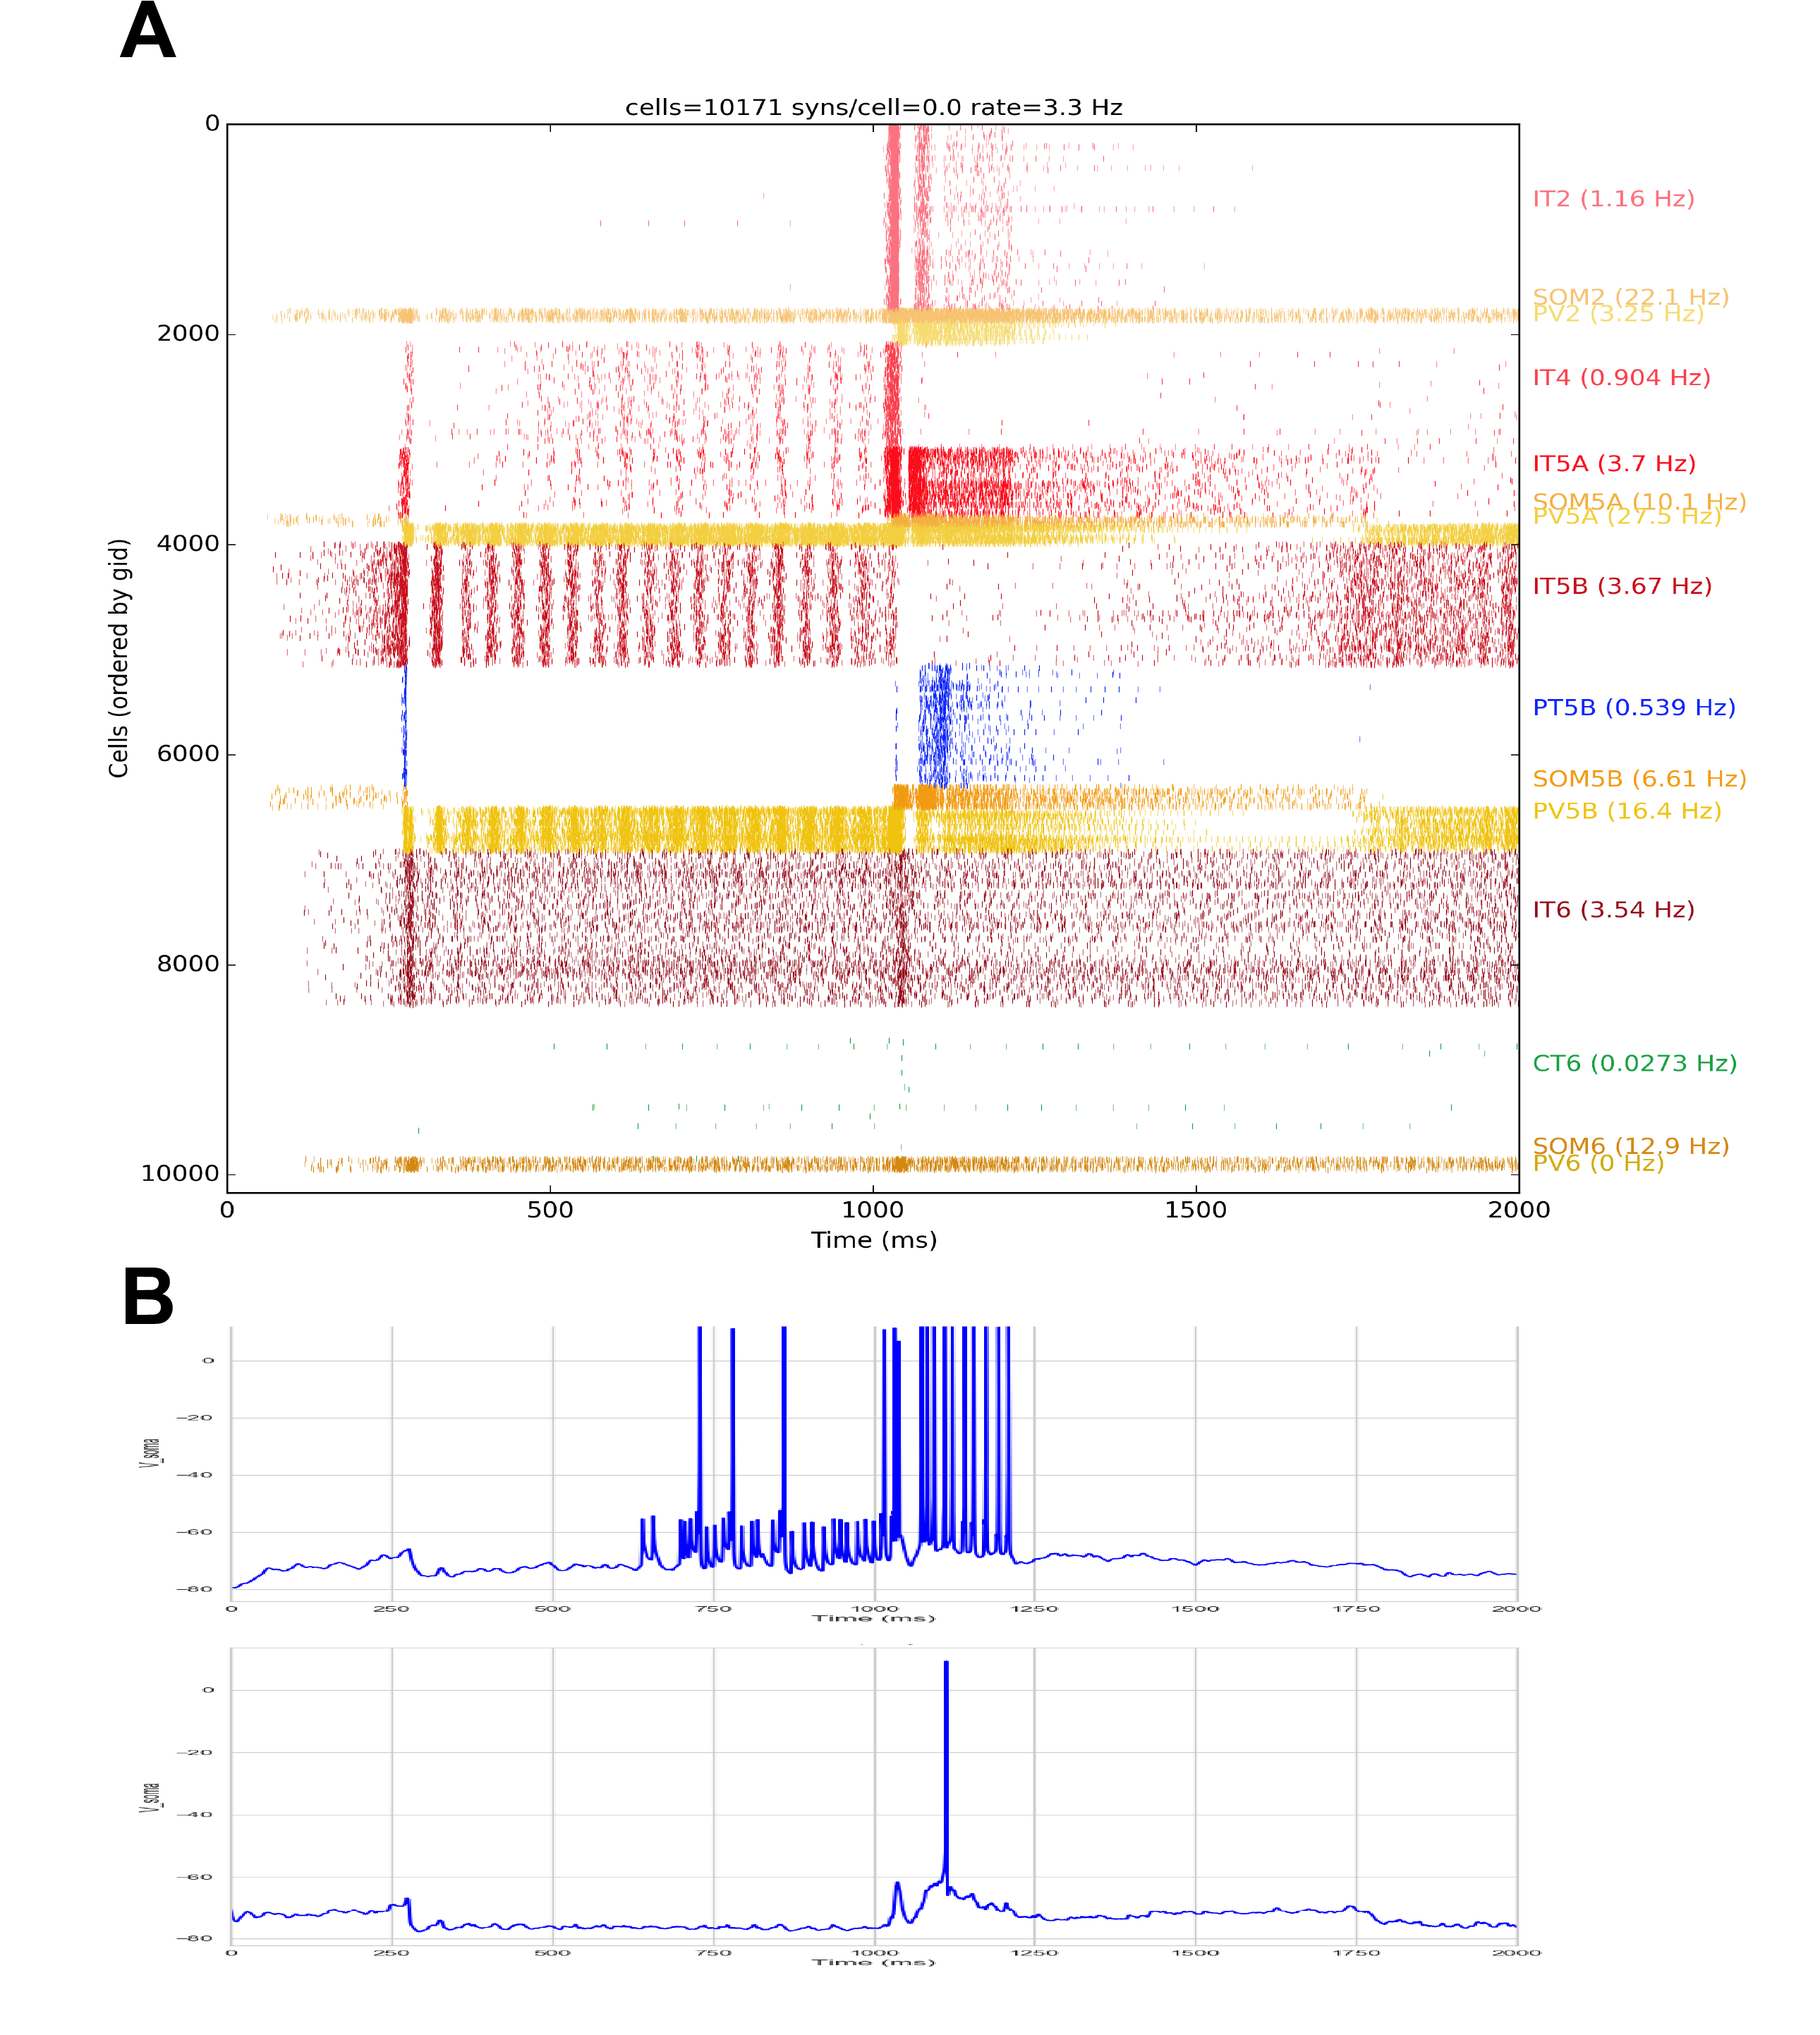
\includegraphics[width=0.7\textwidth]{figs/IT_mode.png}
\caption{{\bf Sensory input with upregulated H-current showing IT-predominant mode (low PT). [INCLUDE CIRCUIT DIAGRAM (GMG SUGGESTION); LABEL LAYERS]}
A) Raster plot. B) IT5A vs P5B example voltage traces.
}
\label{fig_IT_mode}
\end{figure}

\note{ C) Information transfer (Granger and/or nTE) between long range inputs, upper layer ITs and L5B PTs.  4) Comparison of stimulus response delay and average firing rate of upper IT vs PT (N = 25 = 5 wiring x 5 input seeds)}

\begin{figure}[!h]  %% bht
\centering
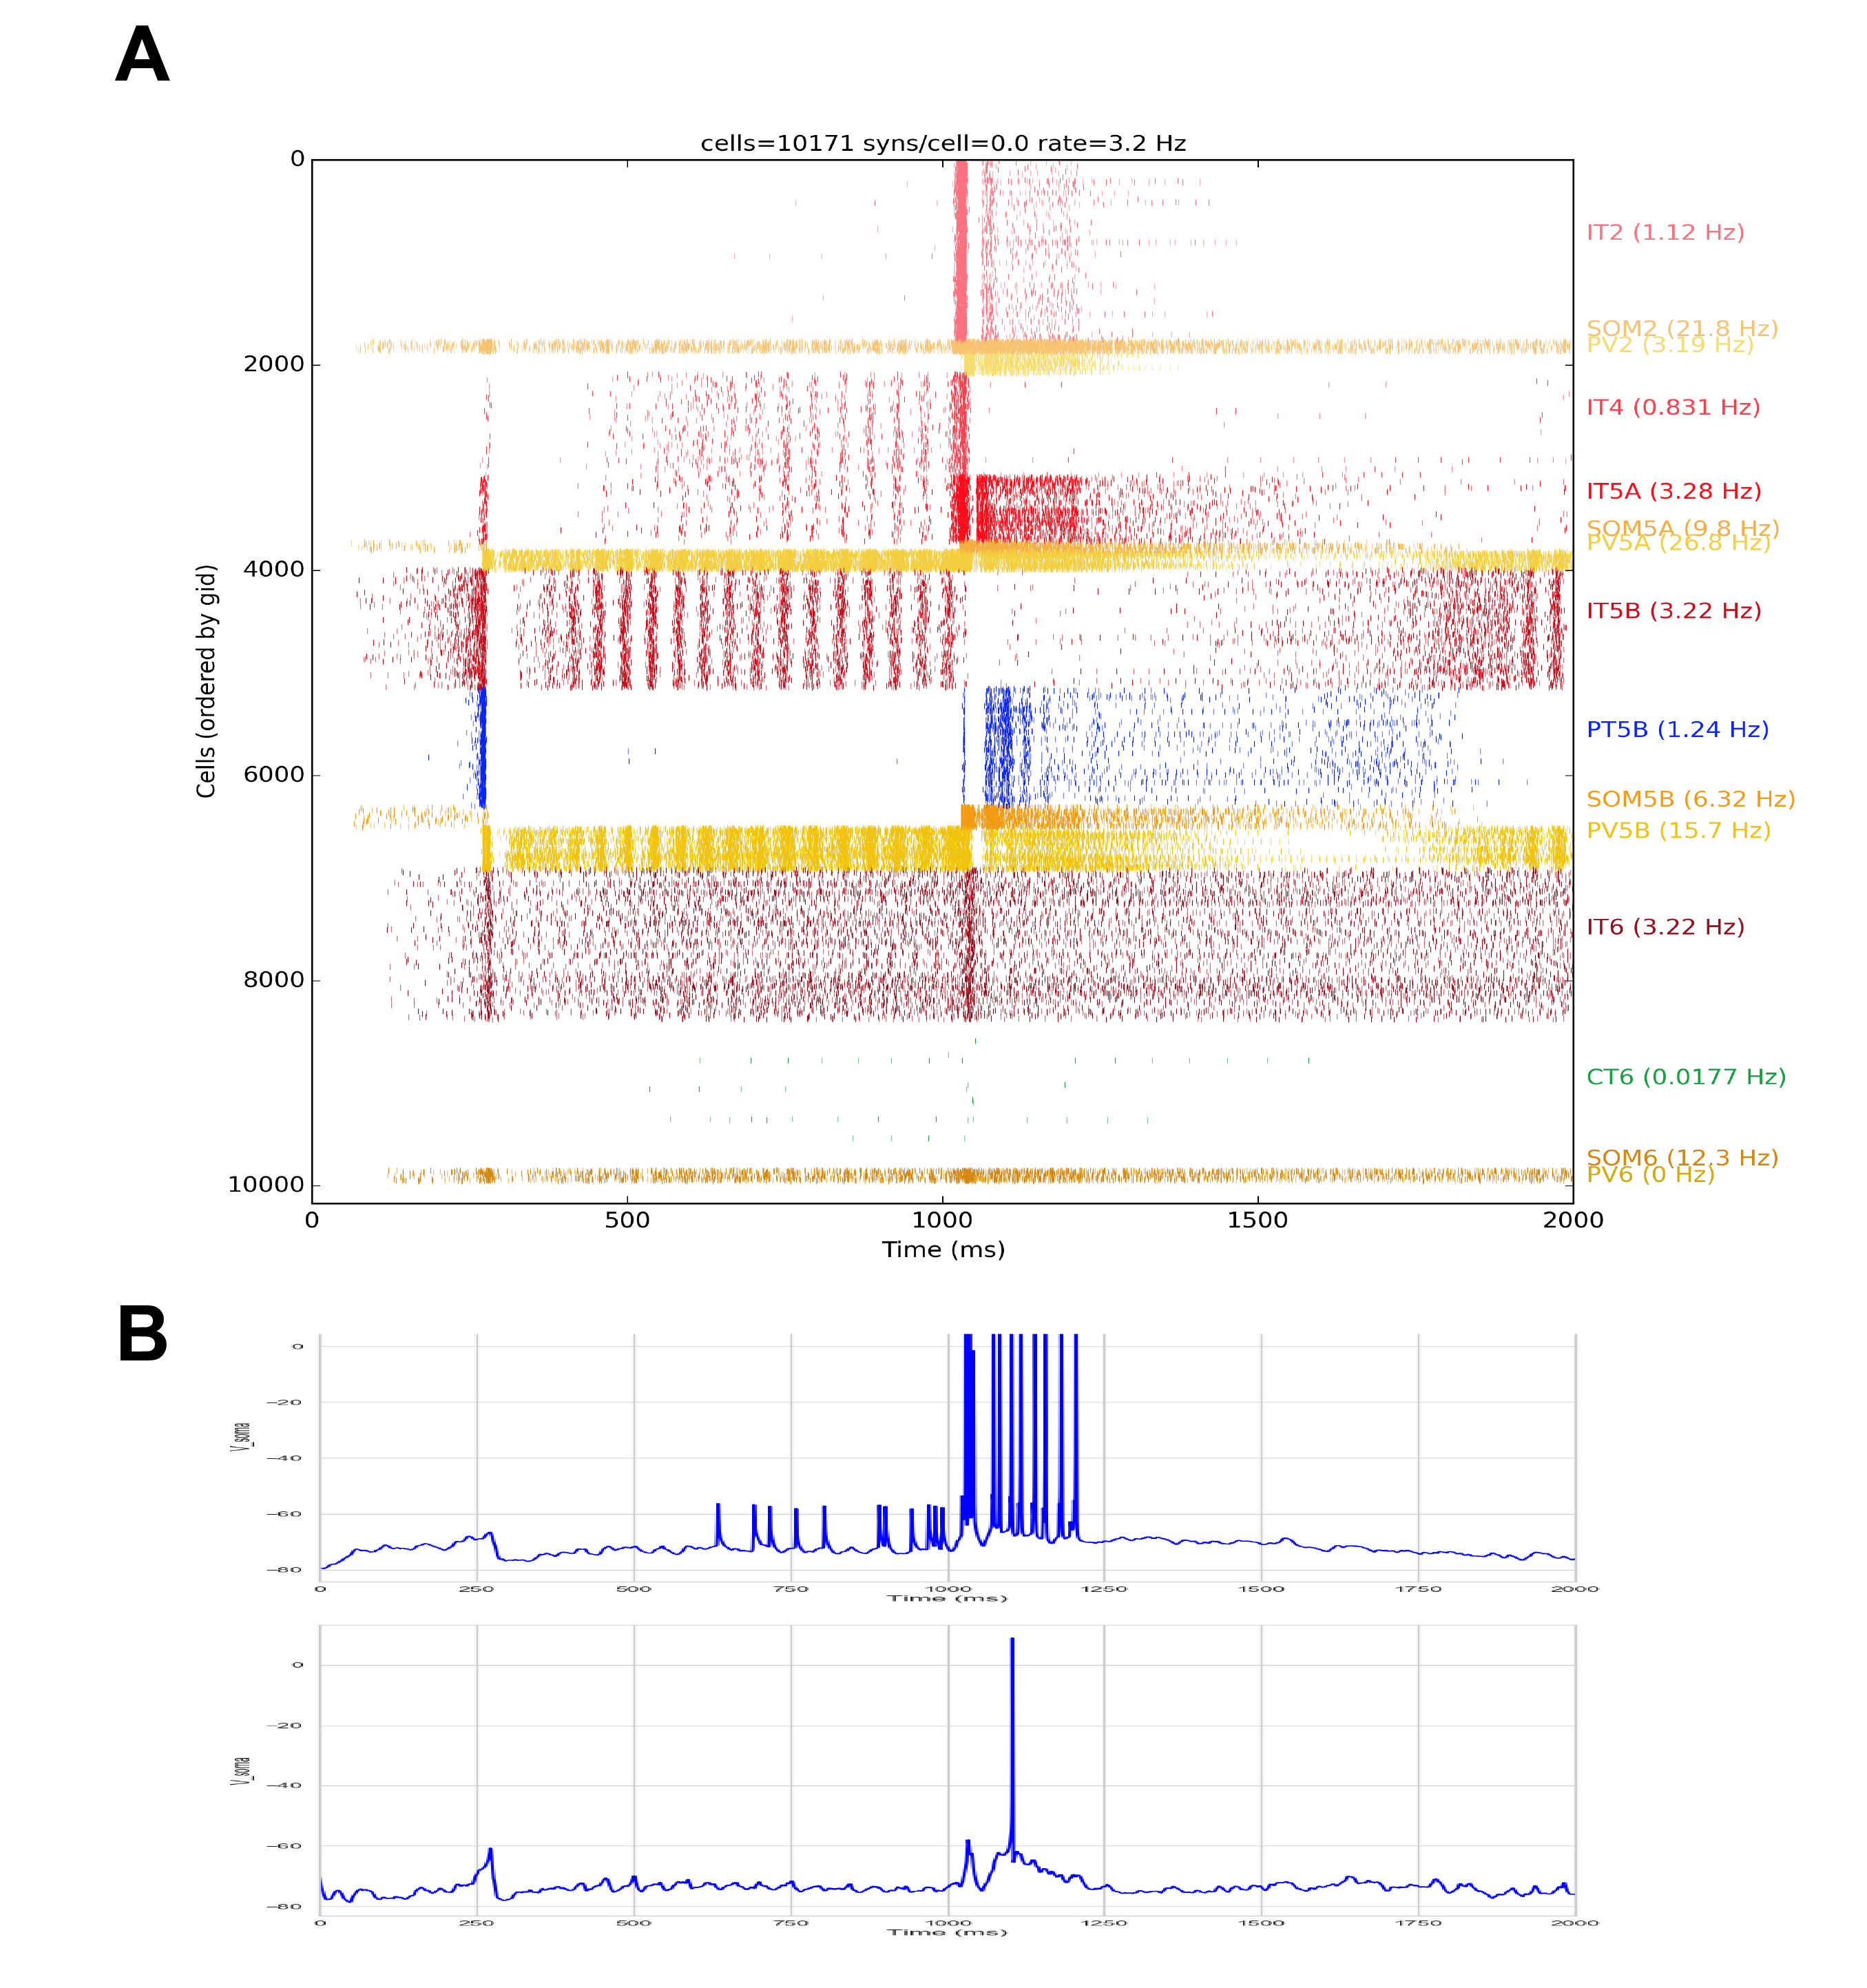
\includegraphics[width=0.7\textwidth]{figs/mixed_mode.png}
\caption{{\bf Sensory input with downregulated H-current showing mixed mode (both IT and PT active}
A) Raster plot. B) IT5A vs P5B example voltage traces. C) Information transfer (Granger and/or nTE) between long range inputs, upper layer ITs and L5B PTs.  4) Comparison of stimulus response delay and average firing rate of upper IT vs PT (N = 25 = 5 wiring x 5 input seeds)
}
\label{fig_mixed_mode}
\end{figure}

Differnet combinations of long-range inputs and H-current levels lead to different modes of operation in M1. Increased rates (20 Hz) in PO, S1 and S2 inputs together with an upregulated H-current favored an IT/CT-predominant mode (with low PT activity) \fref{fig_IT_mode}. The same long-range input levels with H-current downregulated lead to a mixed mode where upper layer IT cells in turn activated PT cells \fref{fig_mixed_mode}. Downregulation of H-current facilitated synaptic integration of inputs and increased PT output activity. This constitutes one of the pathways that can generate corticospinal output: sensory-related inputs projecting to superficial IT neurons in turn exciting PT cells.

\note{Pathways characterized by comparing temporal activation and firing rate of IT vs PT (include example traces); and information flow from upper layers to PT with nTE and/or Granger.}


%%%%%%%%%%%%%%%%%%%%%%%%%%%%%%%%%%%%%%%%%
%% Motor-related pathway and H-current modulation
\subsection{Motor-related pathways and H-current modulation}

\begin{figure}[!h]  %% bht
\centering
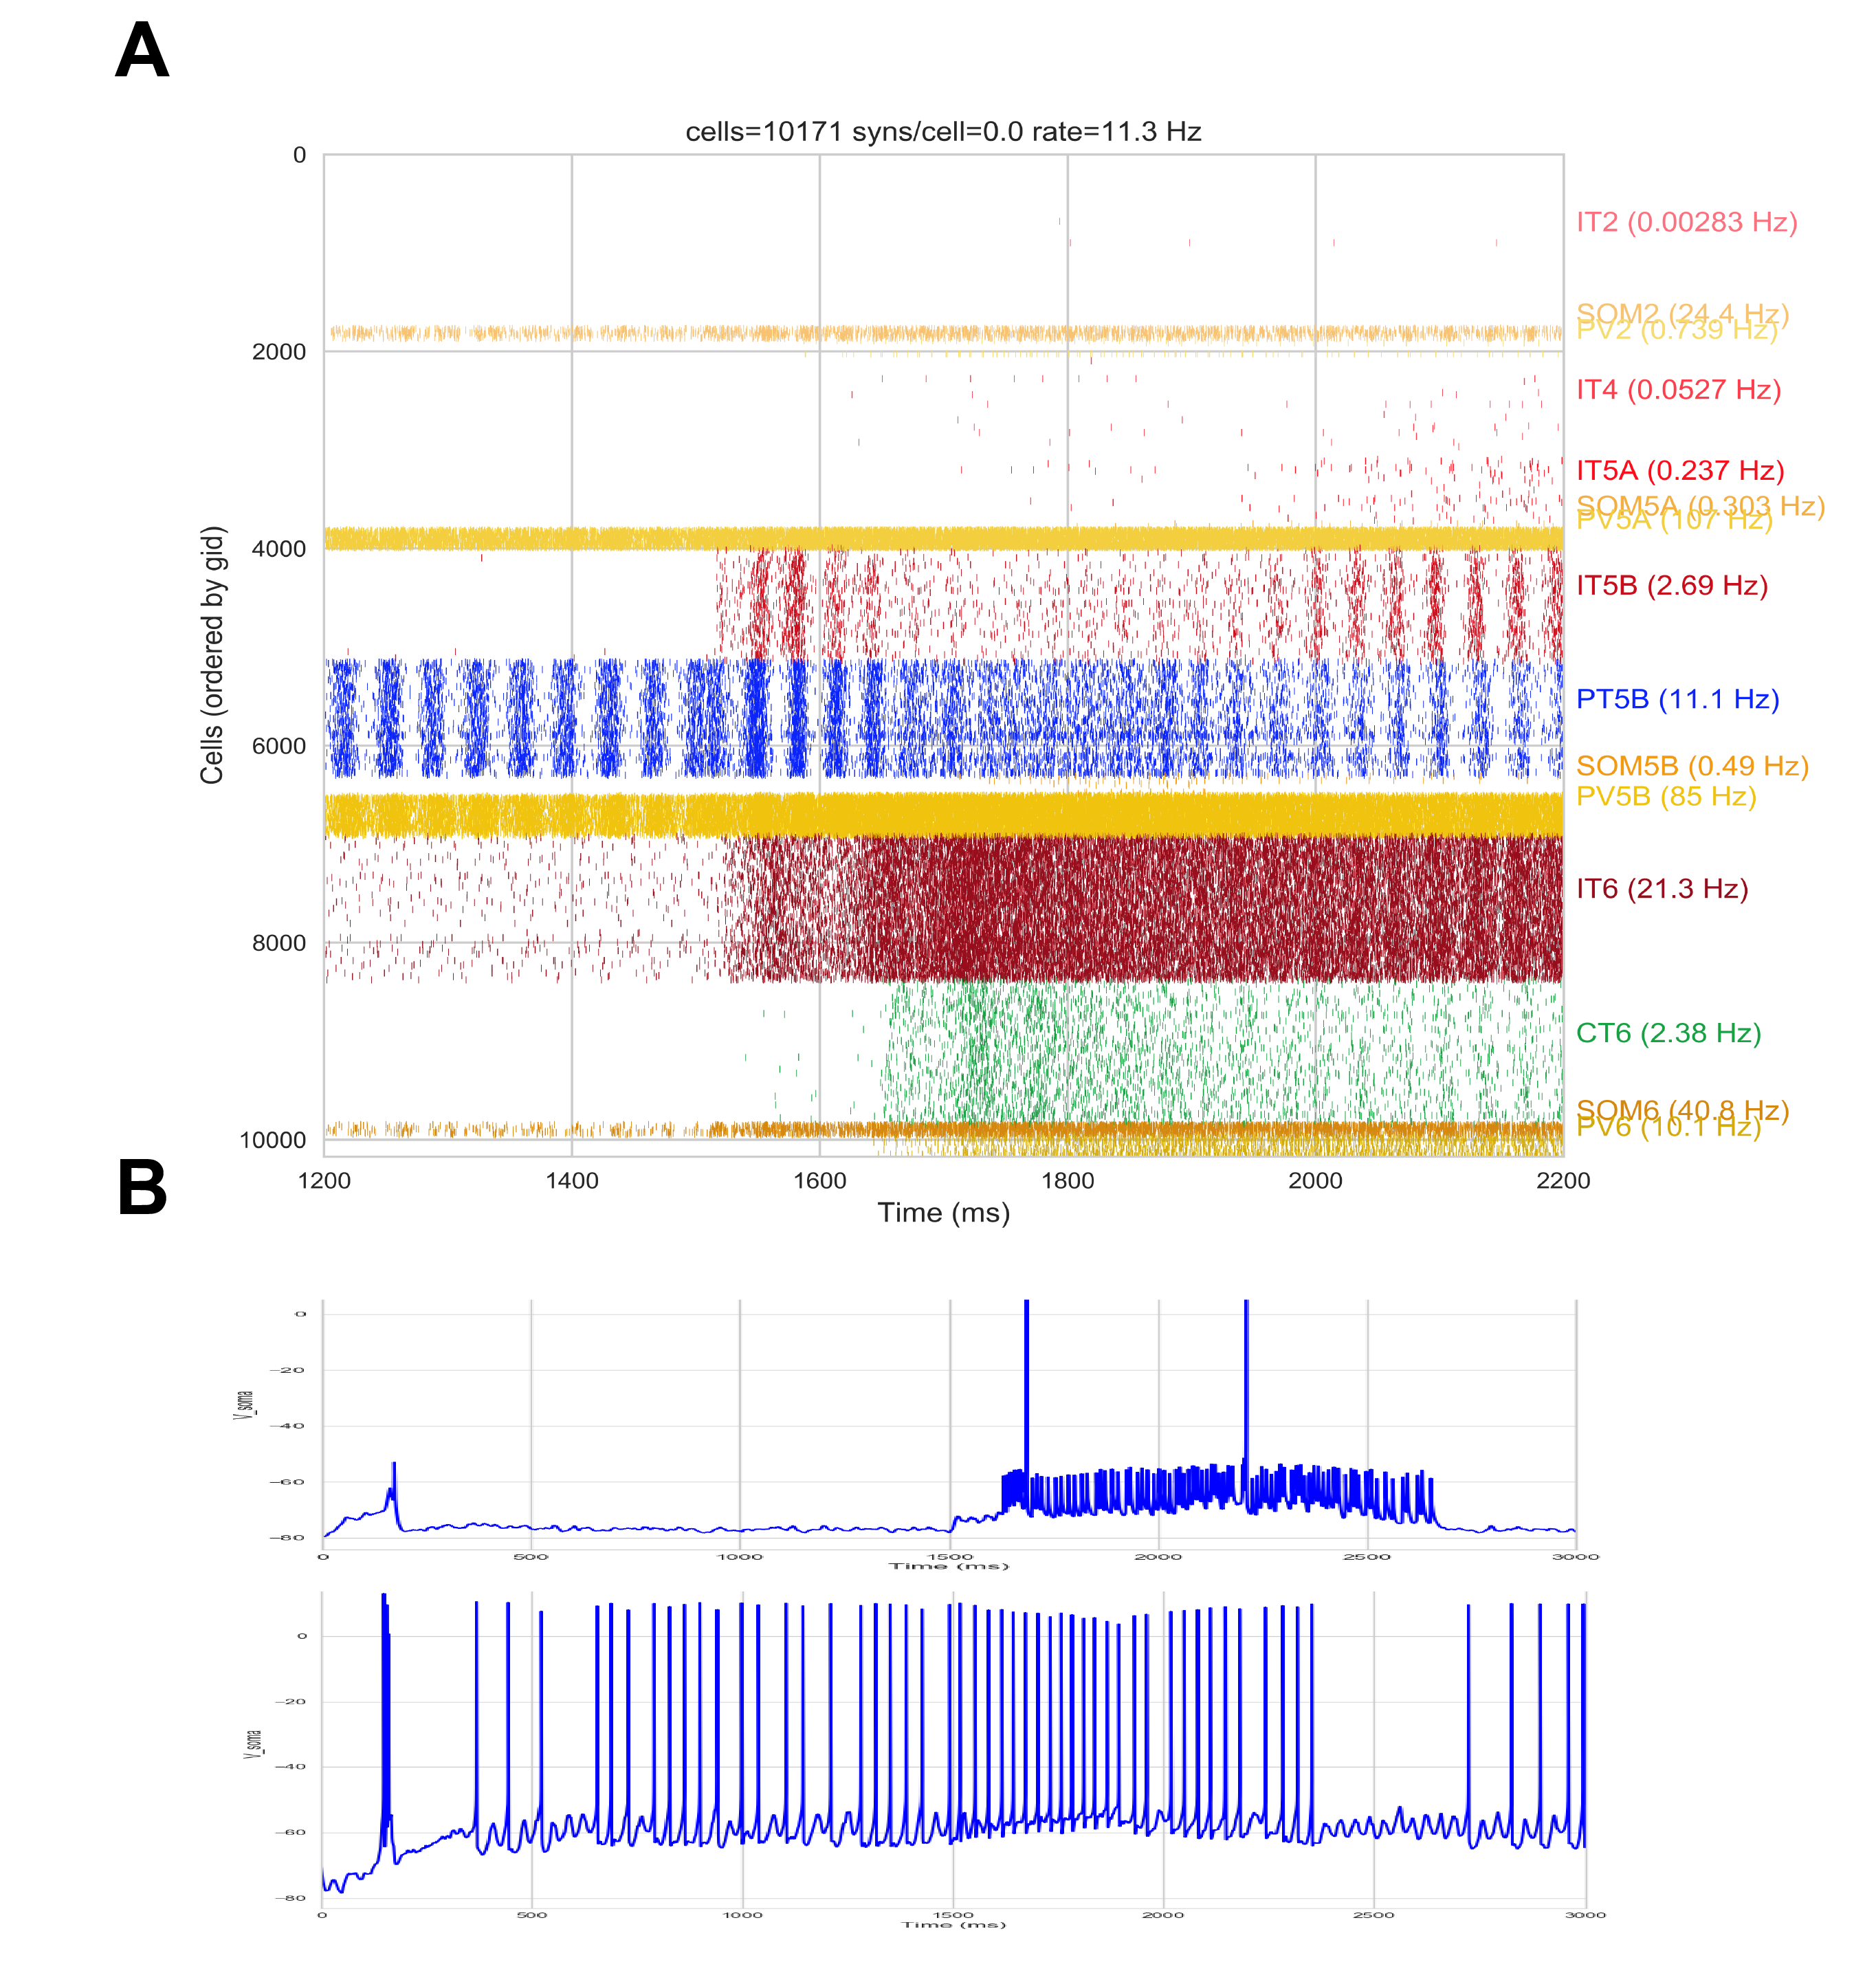
\includegraphics[width=0.7\textwidth]{figs/PT_mode.png}
\caption{{\bf Motor input with downregulated H-current showing PT-predominant mode.}
A) Raster plot. B) IT5A vs P5B example voltage traces. 
}
\label{fig_PT_mode}
\end{figure}

\note{C) Information transfer (Granger and/or nTE) between long range inputs, upper layer ITs and L5B PTs.  4) Comparison of stimulus response delay and average firing rate of upper IT vs PT (N = 25 = 5 wiring x 5 input seeds)}

Increased activation of VL, cM1 and M2 inputs with downregulated H-current promoted a PT-predominant mode \fref{fig_PT_mode}. This evidences a second pathway that can result in corticospinal output: motor-related inputs bypassing upper M1 layers and directly projecting to PT cells. As with sensory-related inputs, upregulation of H-curerent in corticospinal cells also decreased their activity.



%% Other results
\note{
\subsection{Other results/predictions (mostly for next paper)}
- Effect of dendritic distribution of synapses (sCRACM data) on circuit dynamics and neural coding (SfN16 poster).

- Map resonance for different layer inputs (SA 4.2); develop test-set (SA 4.3); 100ms input to different layers, freqs and phases; measure resonance, constructive/destructive interference

- Present time-varying signals to networks (SA 4.4); 2 time-varying signal (different target cells and spectral properties), separate and simultaneously to L2/3; measure rates, LFP, nTE, Granger in L5A IT and L5B PT; how is signal transformed?

 - Wiring perturbations (structure-function relations) (SA 4.5); L2/3 strong effect; L2/3->L5 hyperconn -> autism
 
- Simultaneous activation of inputs e.g. thalamus and vS1 -> vM1\cite{Hook15}

- Study more in depth effect of H-current on spatial and temporal integration L2/3 inputs to PT (already have results reproducing figs 4, 7, 8, 9 and 11 from Sheets, 2011)

- Evaluate STR-SPI transformation hypothesis (rate vs temporal coding) via temporal-variability measures.

- Reproduce data in Dembrow, 2015: IT dendrites functioned as temporal integrators, particularly responsive to dendritic inputs within the gamma freq range (40 –140 Hz); PT dendrites acted as coincidence detectors, responding to spatially distributed signals in a narrow time window.

- Study role of interneurons: interlaminar disynaptic interactions (E->I->E); replicate ratios in Yamawaki,2015.

- Compare oscillations in different layers (eg. alpha=suppress -- use Lakatos paper, gamma=info flow, beta=resting?)

- Study correlations and synchrony: spike-triggered average; auto- and cross-correlations between spike trains; joint peri stimulus time histograms; cross-level coupling (CLC); spike train synchrony measures; Pairwise Phase consistency (PPC)

- Study effect of low vs high frequency synaptic inputs on network (the network analogous of cell synaptic resonance in apical dendrites for high frequencies)
}

